\documentclass[12pt]{article}

\usepackage{fullpage}
\usepackage{multicol,multirow}
\usepackage{tabularx}
\usepackage{ulem}
\usepackage{graphicx}%Вставка картинок правильная
\usepackage{float}%"Плавающие" картинки
\usepackage{wrapfig}%Обтекание фигур (таблиц, картинок и прочего)
\usepackage[utf8]{inputenc}
\usepackage[russian]{babel}

\begin{document}

\section*{Лабораторная работа №\,8 по курсу дискрeтного анализа: жадные алгоритмы}

Выполнил студент группы 08-307 МАИ \textit{Дегтярев Денис Андреевич}.

\subsection*{Условие}

На координатной прямой даны несколько отрезков с координатами Li, Ri. Необходимо выбрать минимальное количество отрезков, которые бы полностью покрыли интервал от 0 до M.

\subsection*{Метод решения}

Данную задачу решал с помощью жадного алгоритма: пока мы не достигнем цели, выполняем. Ограничитель: условие не выполнится, тк цель не достижима. 
Оптимальный отрезок: тот, у которого максимальная правая часть и левая часть меньше правой записанного элемента сверху.
Тогда возможно, что в конечном итоге мы доберемся до m.

\subsection*{Описание программы}

Создаем структуру отрезка и начинаем перебирать каждый из отрезков на каждой итерации. Если отрезок локально оптимальный(покрывает большую часть отрезка m и соединен с 
предыдущим отрезком из вектора), то мы его добавляем вверх вектора и переходим на следующую итерацию. Если таких нет: критерий останова, условие не выполняется.

\subsection*{Дневник отладки}

    - WA как я понял происходил из-за переопределения оператора < для моей структуры, однако почему он так странно работал, не понятно...


\subsection*{Тест производительности}

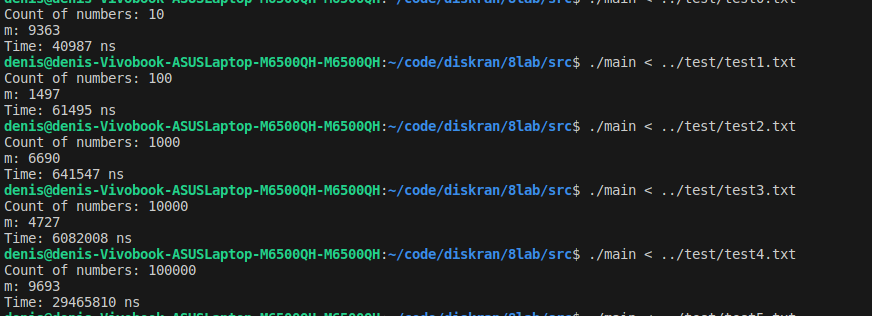
\includegraphics[width=7in]{test.png}

\subsection*{Недочёты}

Недочетов не должно быть... Реализовывал все добросовестно.

\subsection*{Выводы}

Выполнив лабораторную работу №8 по курсу «Дискретный анализ», я изучил
жадный алгоритм и убедился, что он помогает решать задачи, где стандартные решения не подходят.

\end{document}
